\documentclass{article}
\usepackage{graphicx}
\usepackage{geometry}
\usepackage{amsmath}
\begin{document}

\section*{Problem statement}
I discretized the system dynamics as:
\begin{equation}
\begin{bmatrix}
\delta_{t+1} \\
\omega_{t+1} \\
\theta_{t+1}
\end{bmatrix}
=
\begin{bmatrix}
I & sI & 0 \\
sM^{-1}(K^I-B^{GG}) & I + sM^{-1}(K^P-D) & -B^{GL} \\
-{B^{LL}}^{-1}B^{LG} & {B^{LL}}^{-1}K^L_t & 0
\end{bmatrix}
\begin{bmatrix}
\delta_{t} \\
\omega_{t} \\
\theta_{t}
\end{bmatrix}
+
\begin{bmatrix}
0 \\
0 \\
{B^{LL}}^{-1}(P^L_t + \epsilon^L)
\end{bmatrix}
\label{eq:sysdyn}
\end{equation}
where $s$ is the step size, $t^*$ is the attack time, and
\begin{equation}
\label{eq:K}
K^L_t =
\begin{cases}
0   & t < t^* \\
K^L & t \ge t^*
\end{cases}
\end{equation}
The goal is to find $t^*$ and $K^L$ given all other variables.
Measurements of the state variables $\delta$, $\omega$, and $\theta$ may be noisy;
all other variables are known exactly.
%Readings of the $P^L_t$ variable may be noisy, all other variables are known exactly.

\section*{Proposed Solution 1: Many Kalman Filters}

This is a naive baseline solution.

Let $K^L$ be an $m\times n$ matrix, and $\alpha$ be a hyperparameter.
For each $(i,j) \in \{1\dots m\}\times\{1\dots n\}$, let
${K^L}^{(i,j)}$ be the matrix with $\alpha$ in the $(i,j)$ position and $0$ everywhere else.
Let $MSE^{(i,j)}$ be the mean squared error of the Kalman filter's state estimate using ${K^L}^{(i,j)}$.
The idea is that $MSE^{(i,j)}$ will be close to zero when the attack occurs between nodes $i$ and $j$, and far away from zero everywhere else.

In practice, this method works well only when $\alpha$ happens to be very close to the true attack parameter.
Minor changes in $\alpha$, however, can cause large changes in the attack's profile,
resulting in a large mean squared error.

\section*{Proposed solution 2: Unscented Kalman Dual Estimation}

This is a slower, but slightly more robust solution.
Augment Equation \ref{eq:sysdyn} so that $K_t^L$ is one of the state variables.
This gives the (non-linear) system
\begin{equation}
\label{eq:modsysdyn}
\begin{bmatrix}
\delta_{t+1} \\
\omega_{t+1} \\
\theta_{t+1} \\
K^L_{t+1}
\end{bmatrix}
=
\begin{bmatrix}
I & sI & 0 & 0 \\
sM^{-1}(K^I-B^{GG}) & I + sM^{-1}(K^P-D) & -B^{GL} & 0\\
-{B^{LL}}^{-1}B^{LG} & {B^{LL}}^{-1}K^L_t & 0 & 0 \\
%-{B^{LL}}^{-1}B^{LG} & 0 & 0 & {B^{LL}}^{-1}\omega_t \\
0 & 0 & 0 & I
\end{bmatrix}
\begin{bmatrix}
\delta_{t} \\
\omega_{t} \\
\theta_{t} \\
K^L_t
\end{bmatrix}
+
\begin{bmatrix}
0 \\
0 \\
{B^{LL}}^{-1}(P^L_t + \epsilon^L) \\
0
\end{bmatrix}
\end{equation}
Now we can solve for $K^L_{t+1}$ using the unscented Kalman filter at the same time that we solve for the state variables.

\subsection*{Solution 2a: sparsity and softmax}
%Solving the system directly results in slow convergence of the $K^L$ variable to the true value and a poor estimate of $t^*$.
Solving the system directly does not take advantage of $K^L$'s inherent sparsity.
A simple way to enforce sparsity is as follows:
after each update step for the UKF,
set $K^L_{t+1} = \text{softmax}(K^L_t)$.
The softmax ensures that only the most important components of the matrix are kept, but that we don't lose important information (e.g. the presence of multiple attacks, or an accidental mistake where the wrong component gets a high initial value).

\begin{figure}
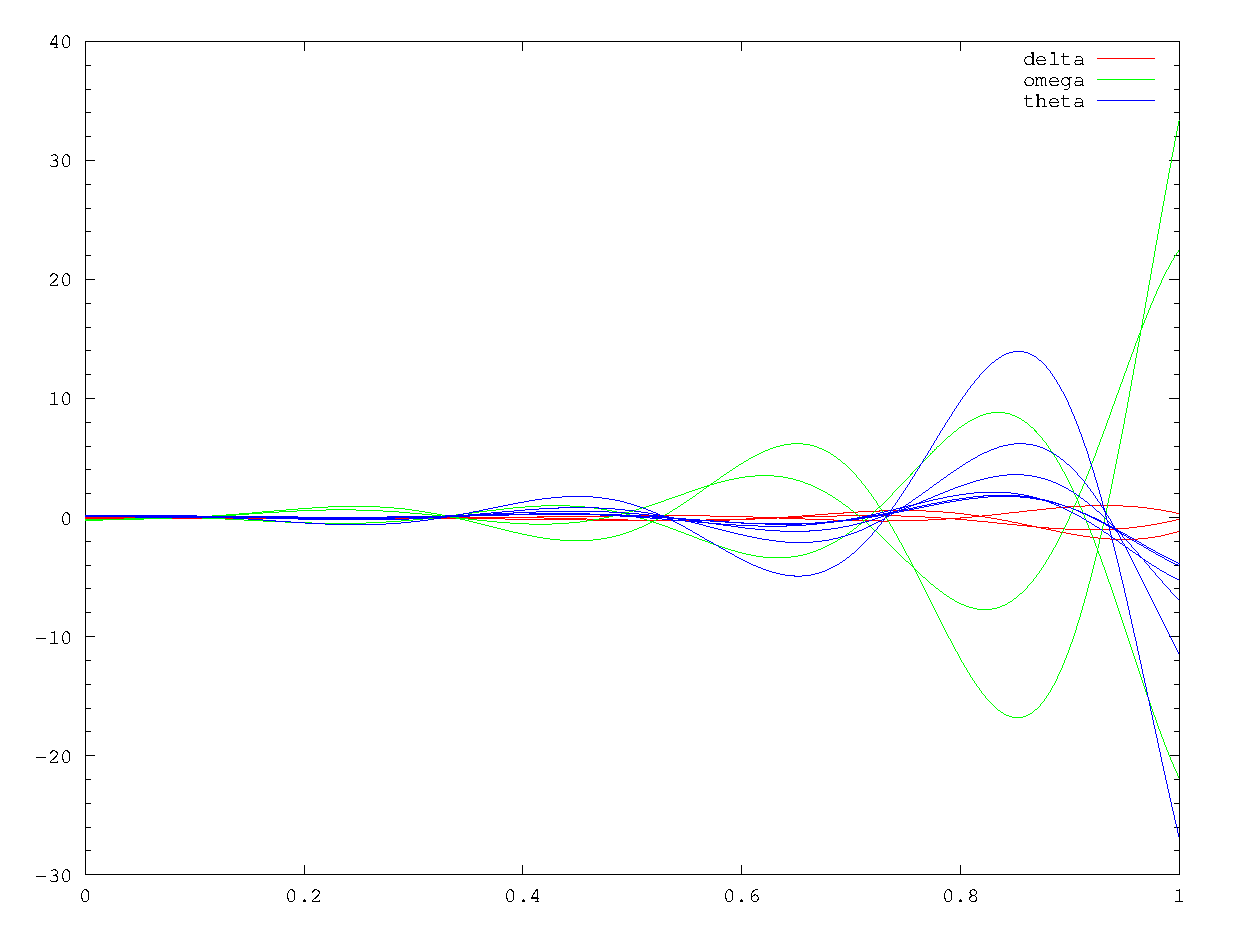
\includegraphics[width=0.3\textwidth]{method2a/example1-states}
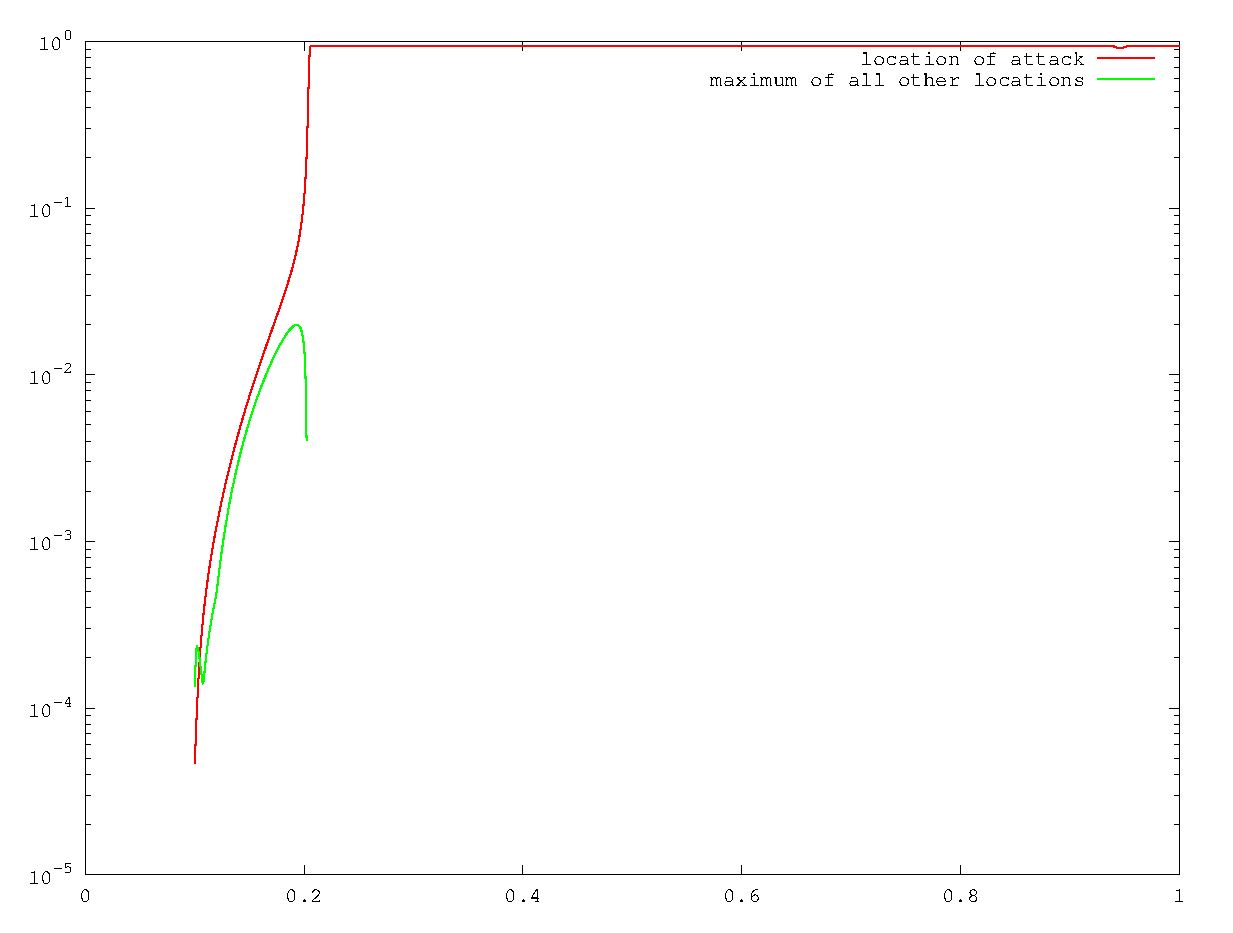
\includegraphics[width=0.3\textwidth]{method2a/example1-K_L}
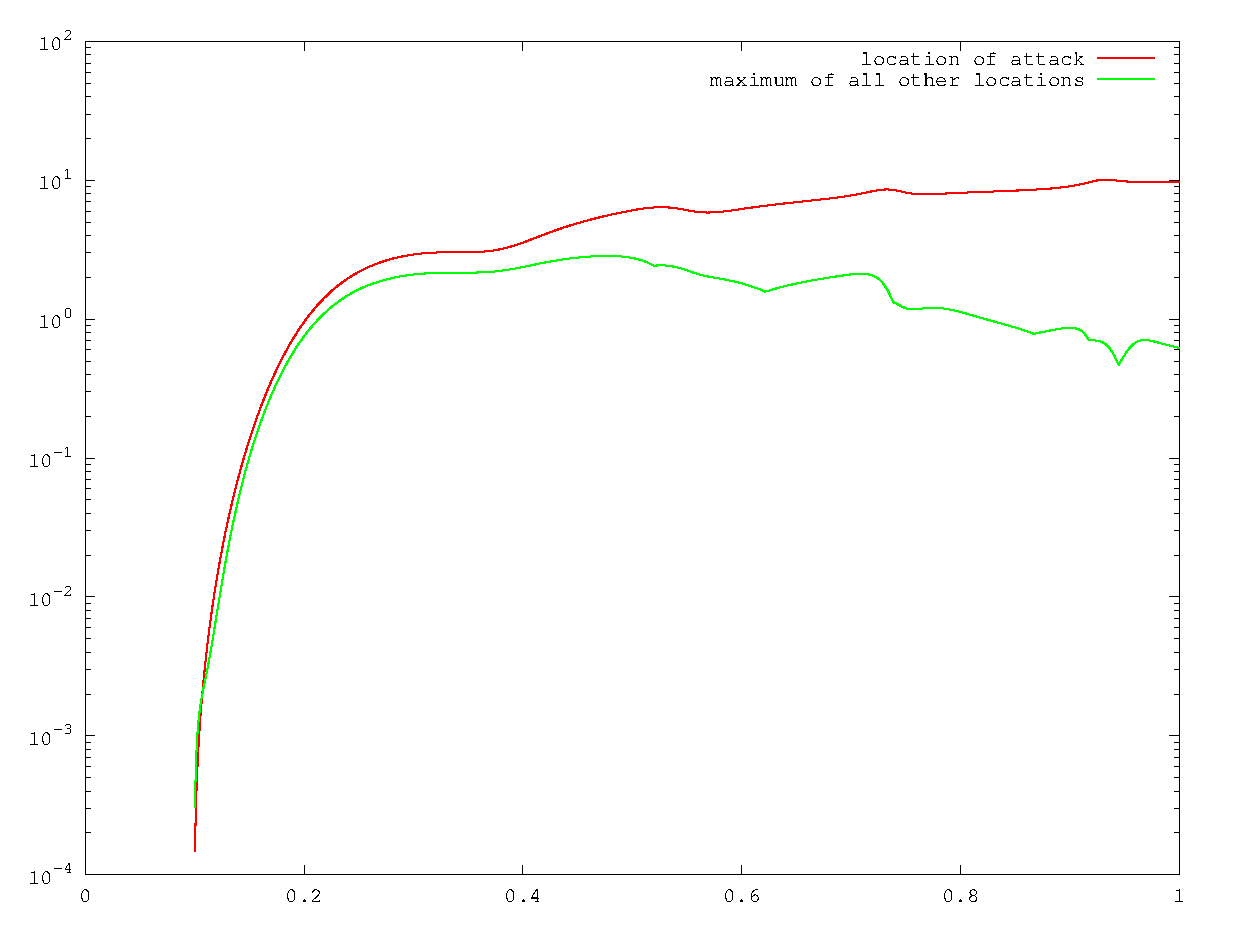
\includegraphics[width=0.3\textwidth]{method2a/example1-K_L-raw}
\caption{
    The results of method 2a on the example with 6 loads and 3 generators.
    The attack occurs at time 0.1.
    (left) The states.
    (center) The estimates of $K^L$ with softmax.
    (right) The estimates of $K^L$ without softmax.
}
\end{figure}

\begin{figure}
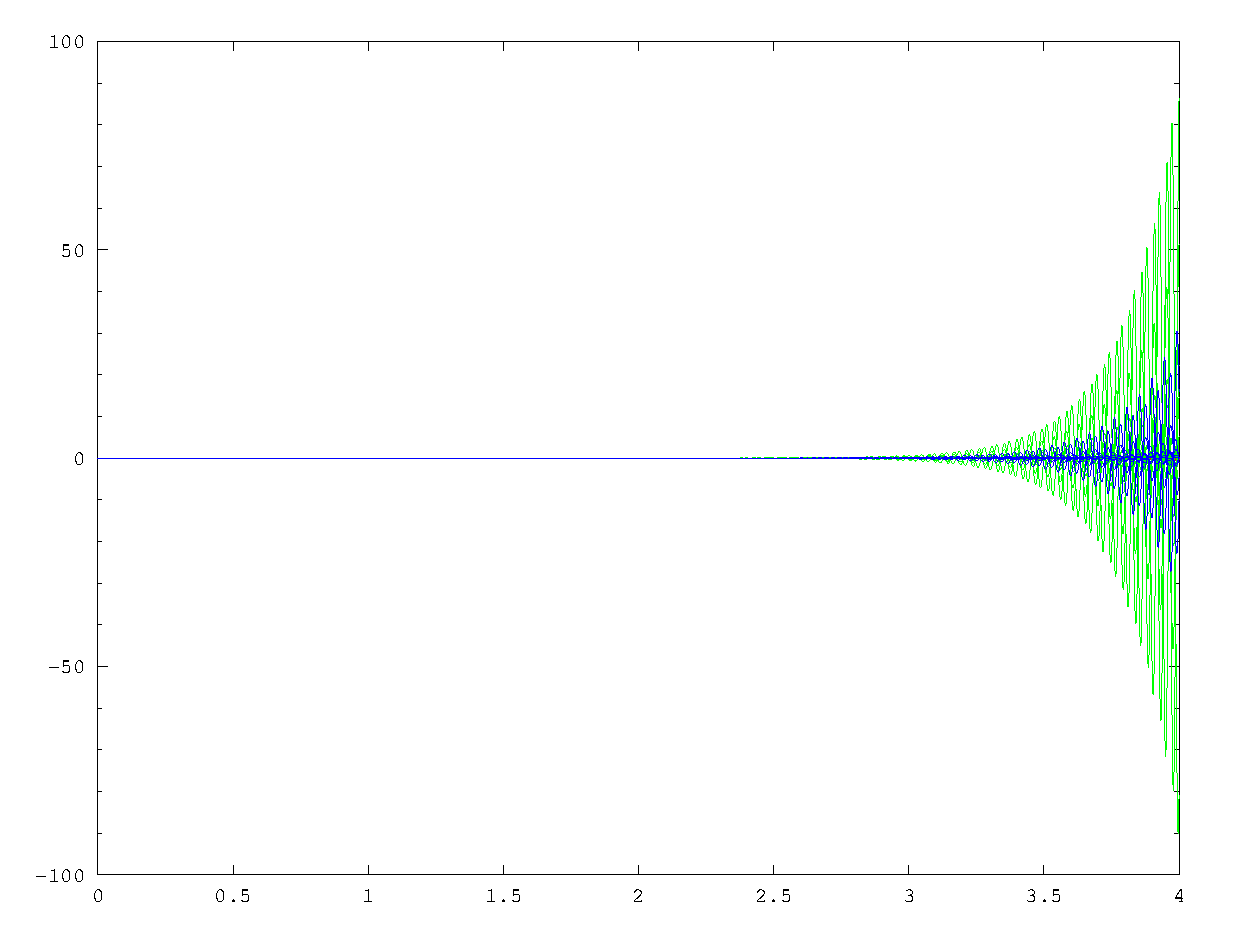
\includegraphics[width=0.3\textwidth]{method2a/random-8x10x25-states}
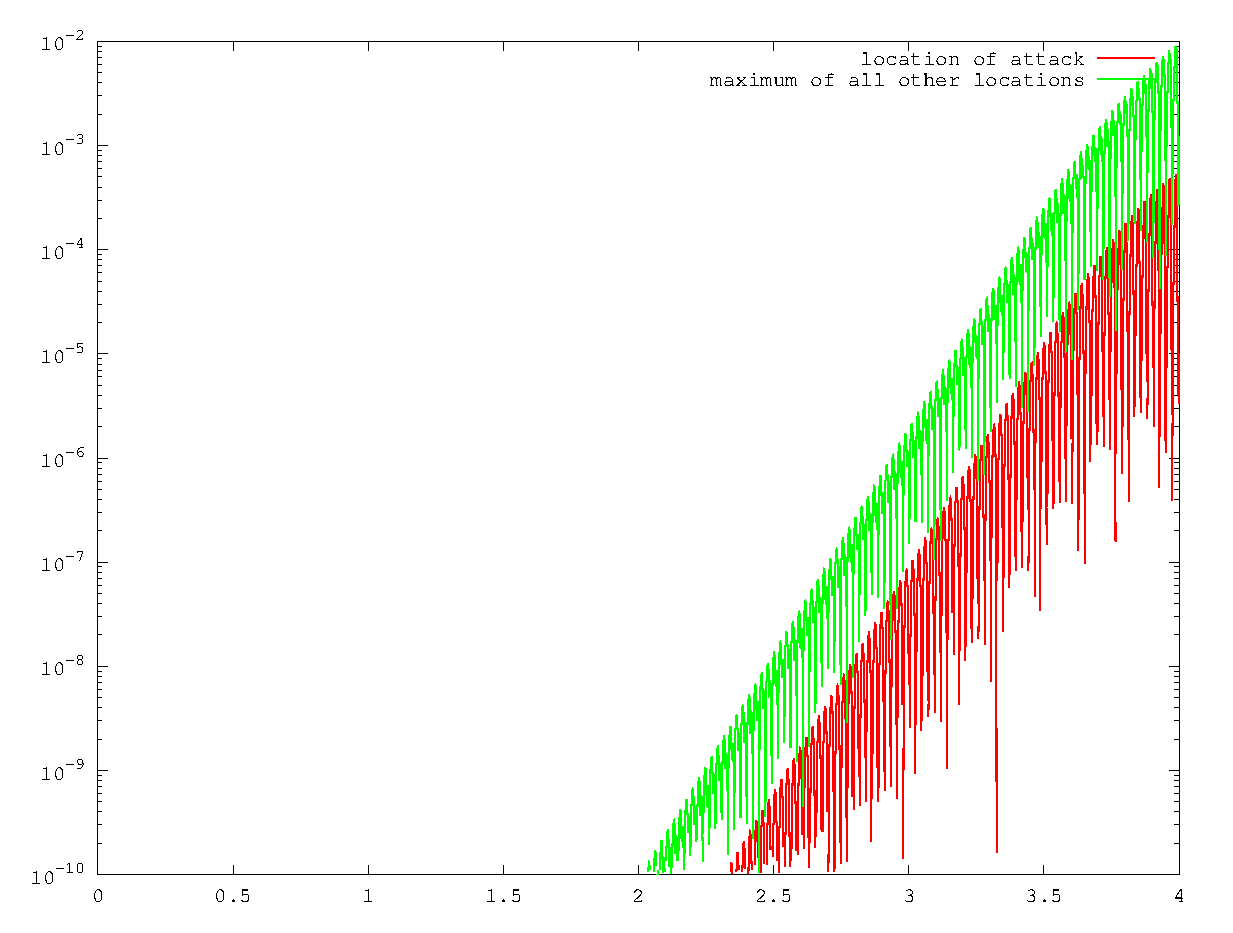
\includegraphics[width=0.3\textwidth]{method2a/random-8x10x25-K_L}
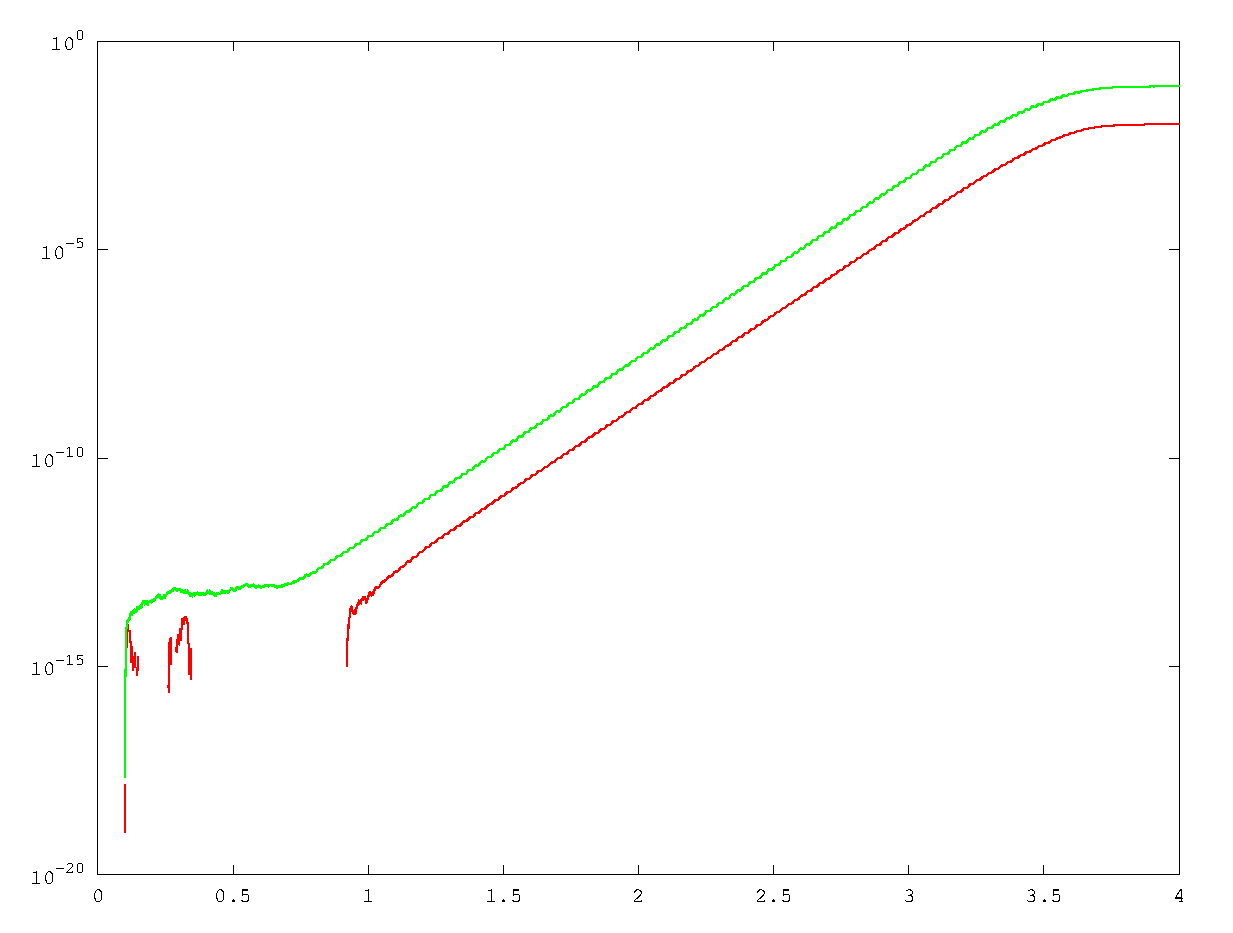
\includegraphics[width=0.3\textwidth]{method2a/random-8x10x25-K_L-raw}
\caption{
    The results of method 2a on a randomly generated power grid with 8 generators and 10 loads.
    The attack occurs at time 0.1.
    (left) The states.
    (center) The estimates of $K^L$ with softmax.
    (right) The estimates of $K^L$ without softmax.
    Without the softmax, we get a better estimate of $t^*$, but a poor estimate of $K^L$.
    With the softmax, the estimate of $t^*$ is delayed, but there is only a small number of non-zero entries in the estimated $K^L$ matrix.
}
\end{figure}

\subsection*{Solution 2b: high variance}
The system dynamics in Equation \ref{eq:modsysdyn} assume that $K_t^L$ is constant for all $t$.
As shown in Equation \ref{eq:K}, however, this is not the case.
$K_t^L$ will be constant everywhere except the attack location.
This means our system dynamics is misspecified precisely at the location of interest.

The Kalman filter accounts for model misspecification by assuming noise in the state transitions.
For computational convenience, this noise is usually assumed to be Gaussian.
In our problem, the noise is clearly non-Gaussian:
for the vast majority of time-steps, we will have essentially zero noise;
but on the time-step of the attack, we will have a large ``spike'' of noise.
In this method, we approximate the non-Gaussian noise with a Gaussian distribution of high variance.
There is a tradeoff when selecting the proper value of the variance.
High variances better capture the time of the attack where the value of $K_t^L$ changes drastically,
but low variances better capture the non-attack times where the value of $K_t^L$ is constant.

\begin{figure}
\centering
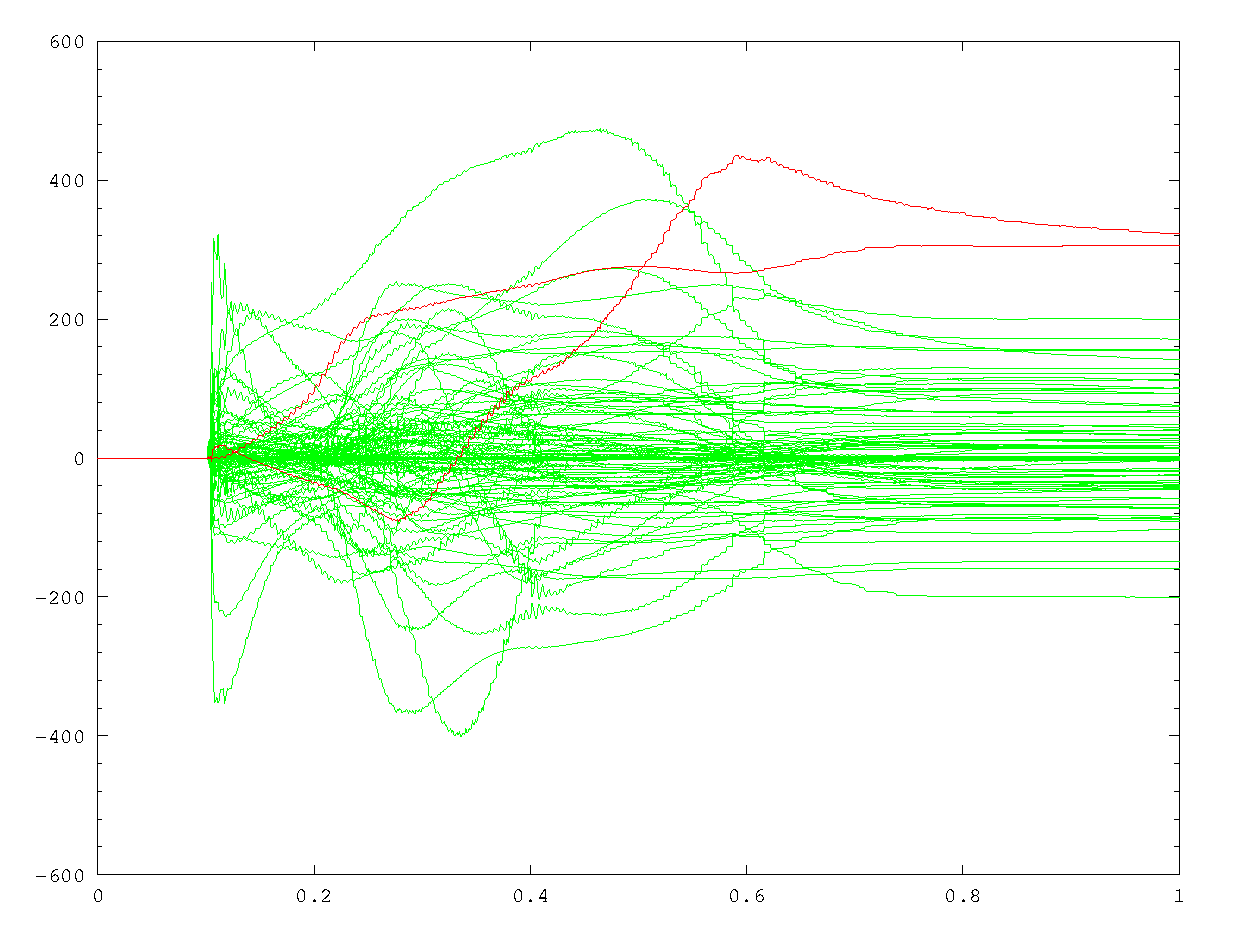
\includegraphics[width=0.5\textwidth]{method2b/highP-6}
\caption{
    The figure above shows the values of $K_t^L$ in a powergrid with 15 generators and 30 loads as estimated using Solution 2b.
    The green lines indicate non-attack locations and the red lines indicate attack location.
    The method correctly identifies attacks when the red lines are significantly higher than the green lines.
    At time $0.1$, two attacks happen simultaneously that destabilize the system.
    The method is able to identify the presence of the attacks immediately,
    but it takes about half a second before the two attacks are correctly identified.
}
\end{figure}

\begin{figure}
\centering
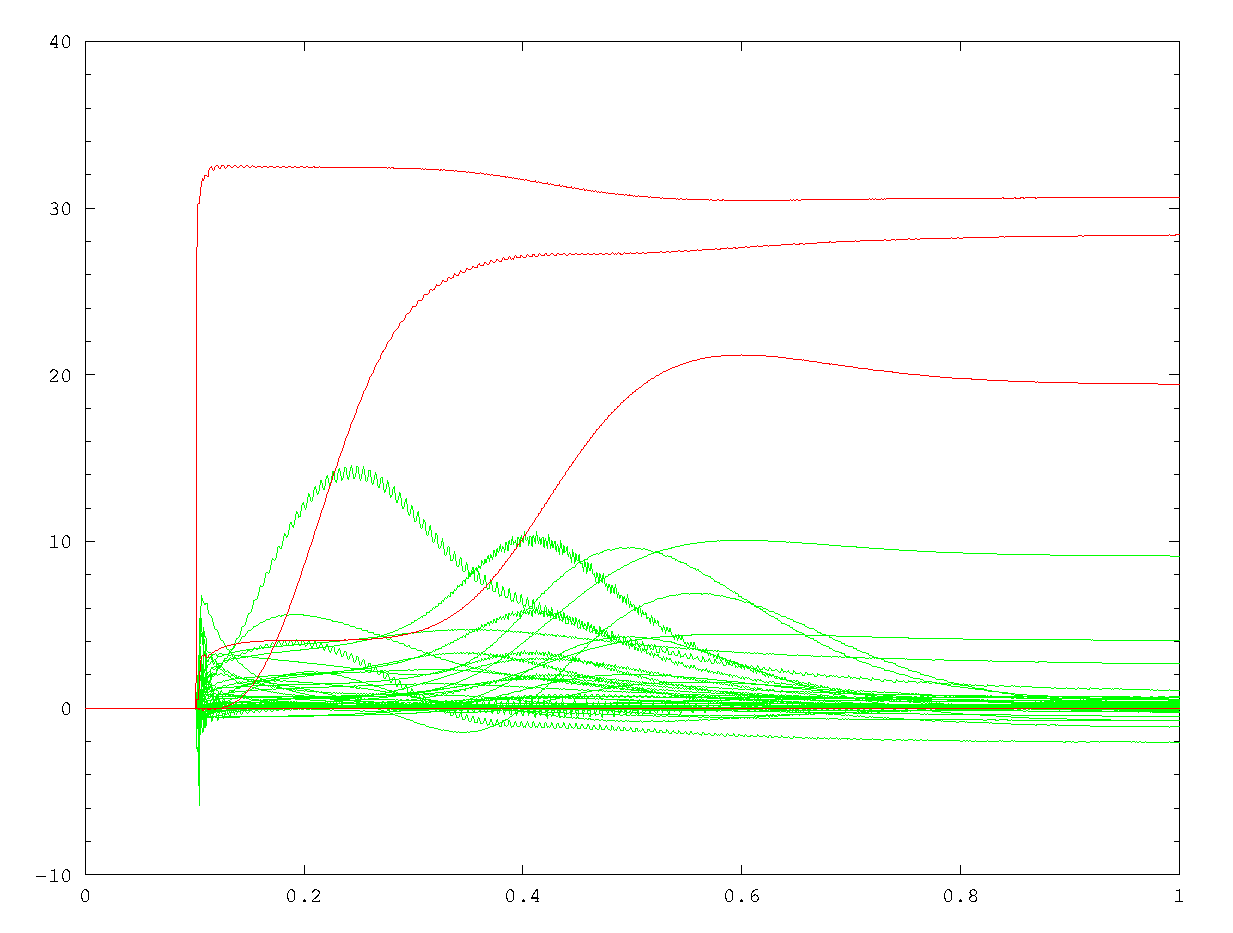
\includegraphics[width=0.5\textwidth]{method2b/highP-6-5attack-zeros1}
%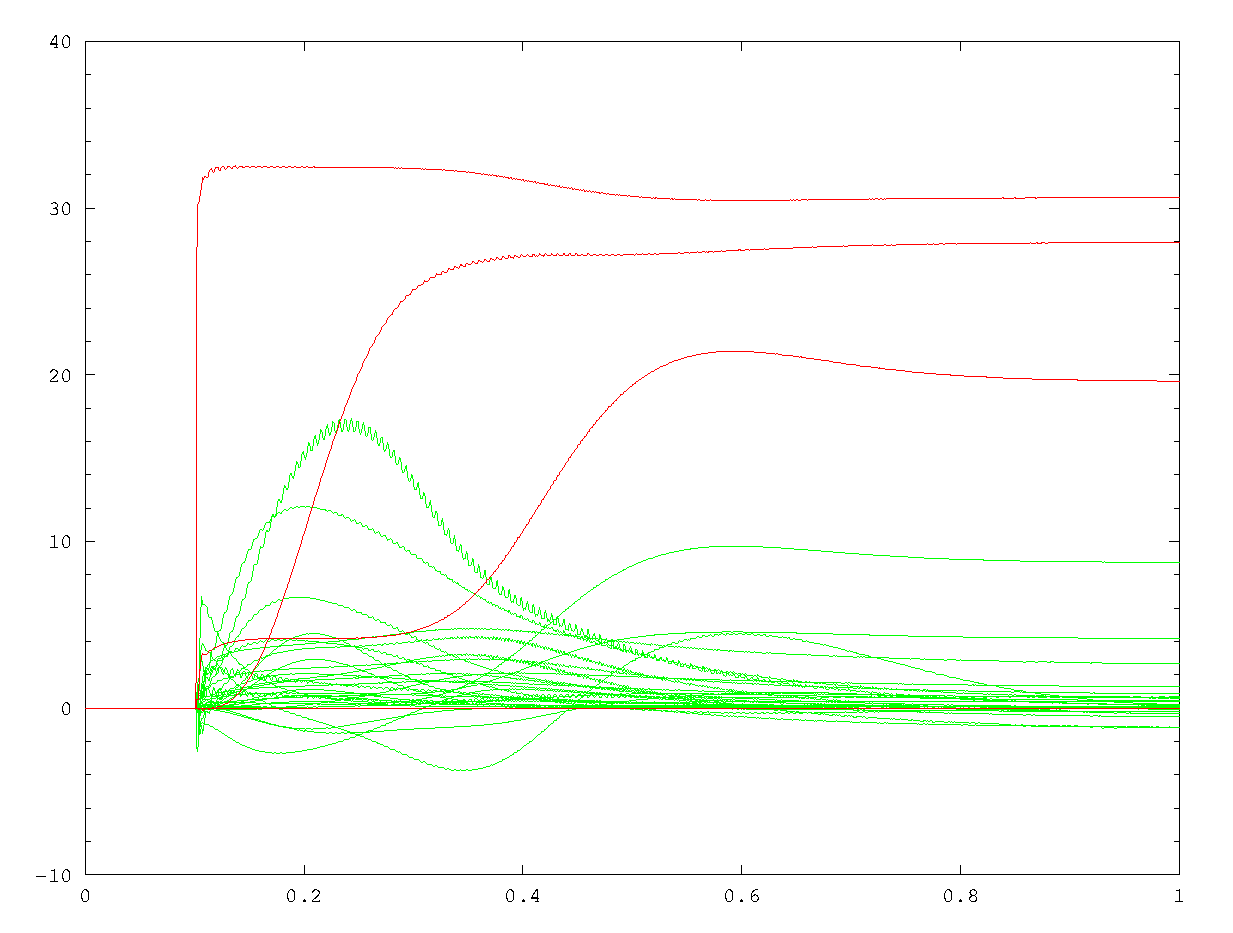
\includegraphics[width=0.3\textwidth]{method2b/highP-6-5attack-zeros2}
%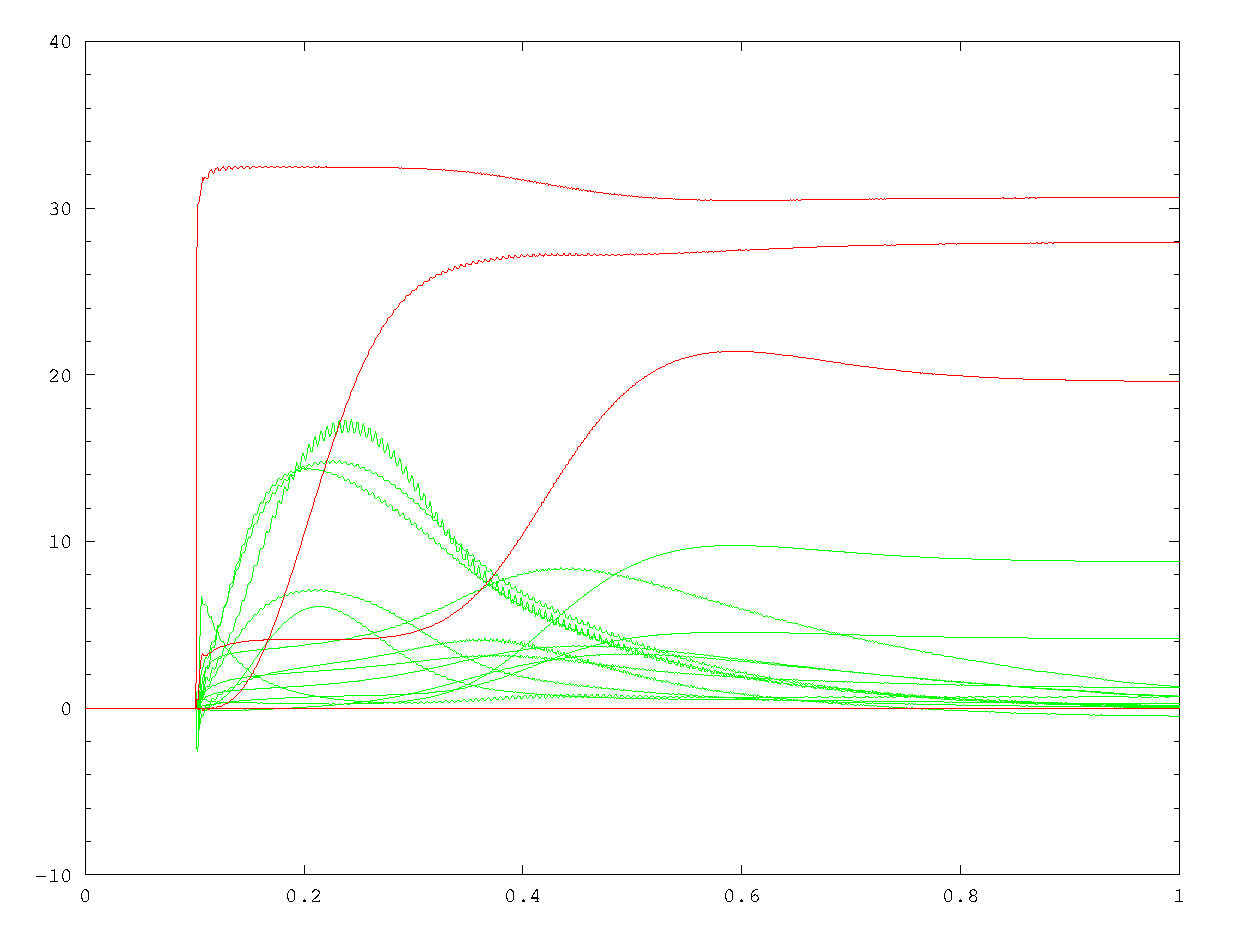
\includegraphics[width=0.3\textwidth]{method2b/highP-6-5attack-zeros3}
%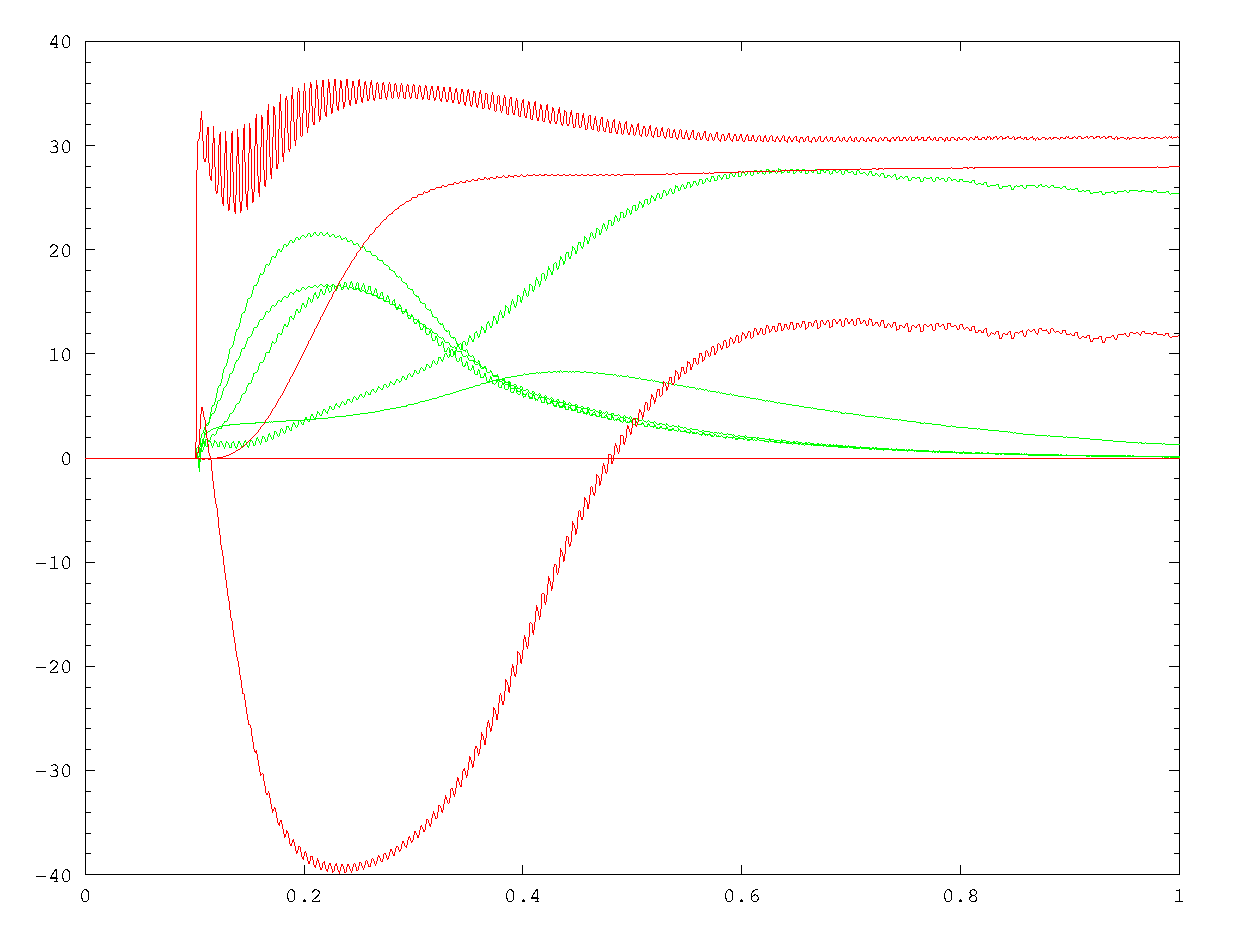
\includegraphics[width=0.3\textwidth]{method2b/highP-6-5attack-zeros4}
%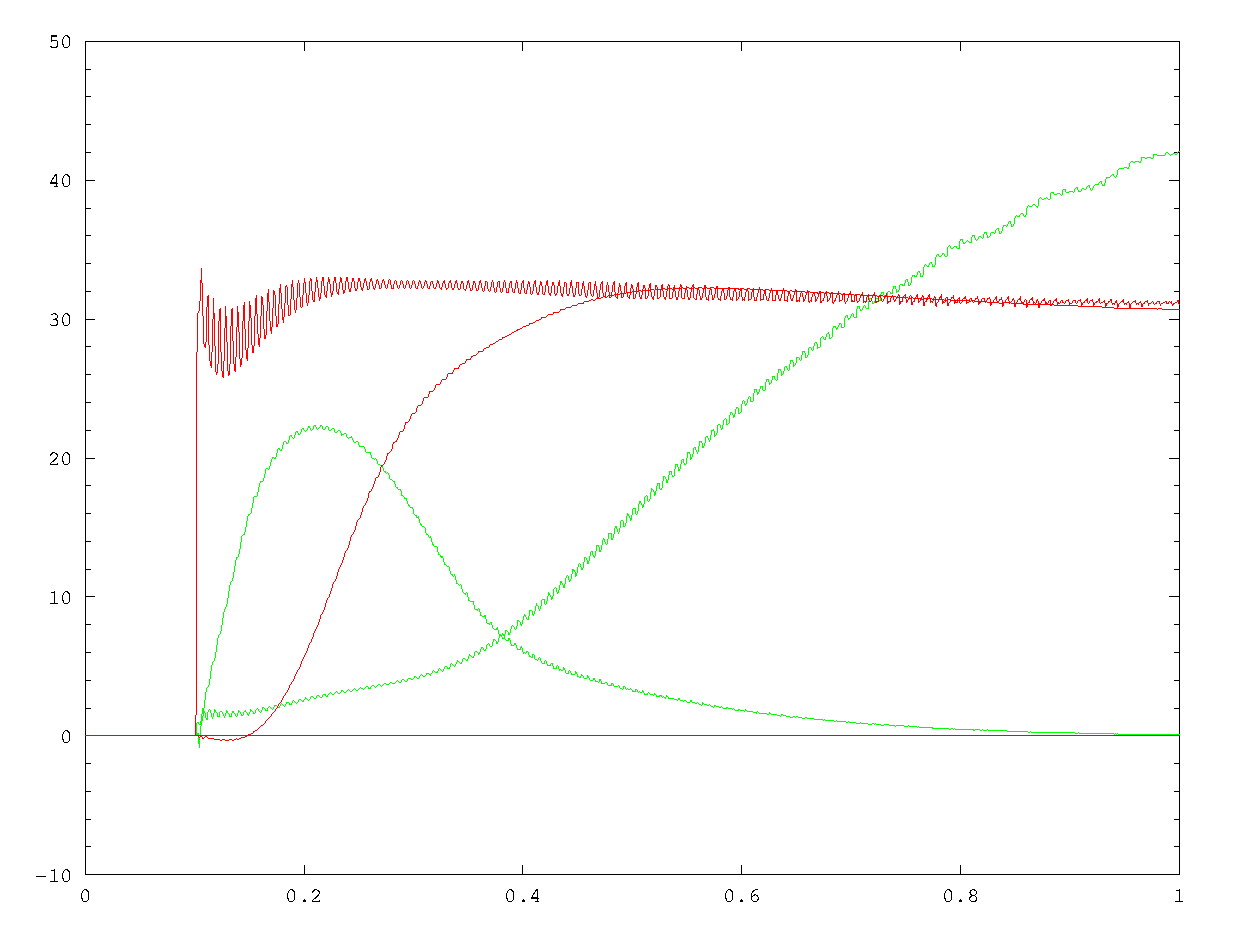
\includegraphics[width=0.3\textwidth]{method2b/highP-6-5attack-zeros5}
%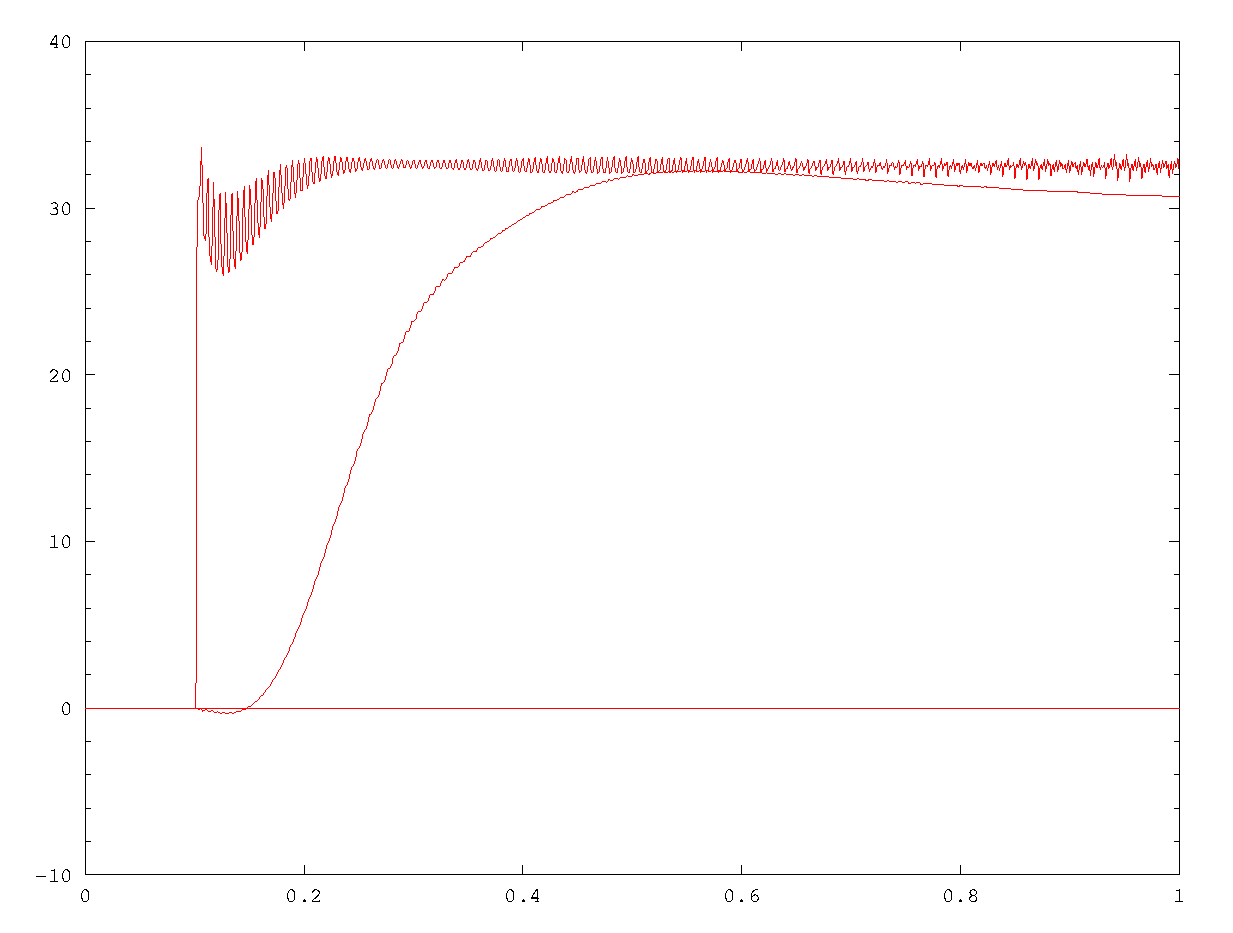
\includegraphics[width=0.3\textwidth]{method2b/highP-6-5attack-zeros6}
\caption{
    The figures above shows the values of $K_t^L$ in a powergrid with 15 generators and 30 loads as estimated using Solution 2b.
    As before, the green lines indicate non-attack locations; the red lines indicate attack locations, and the attack occurs at time 0.1.
    In this example, 5 attacks occur simultaneously.
    Solution 2b is only able to identify 3 of those attacks,
    but this is sufficient.
    The attacker needs all 5 attacks to be present to destabilize the system.
    Removing any one of the attacks returns the system to a stable state.
}
\end{figure}
\end{document}
